\section{Separación de convexos}
\newcommand{\aaa}{\textbf{\emph{a}}}
\newcommand{\bbb}{\textbf{\emph{b}}}
\newcommand{\uu}{\textbf{\emph{u}}}

En esta sección introducimos algunos resultados sobre separación a partir del teorema minimax, teorema \ref{MinMax}. En general, estos nos aportan herramientas para poder concluir cuándo dos subconjuntos convexos pueden ser separados mediante un hiperplano. En la siguiente figura \ref{prueba} vemos un ejemplo sobre la situación en la que nos encontramos. \\

Exponemos un resultado sencillo en el que solo involucramos un conjunto.
\bigskip
\begin{teoremaBox}\label{sep1}
Dado $ N \in \NN $, sea $ C \subset \RR^N $ convexo y definimos
\[
\delta := \inf\{ \norm{\ccc}: \ccc \in C \}.
\]
Entonces, existe $ \xx_0 \in \RR^N $ tal que 
\[
\ccc \in C \Longrightarrow \delta \leq \langle \xx_0,\ccc\rangle.
\]
\end{teoremaBox}

\begin{figure}[h!]
	\begin{center}
		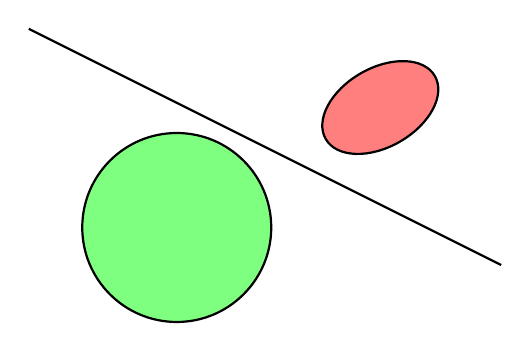
\begin{tikzpicture}[thick,fill opacity=0.5]
		\filldraw[fill=red][rotate = 30] (0:4cm) ellipse (8mm and 5 mm);
		\filldraw[fill=green] (1cm:1cm) circle (12mm);
		\draw (-1,3) -- (5,0);
		%\node at (0.9cm,0.6cm) {\large A};
		%\node at (3.5cm,2.1cm) {\large B};
		\end{tikzpicture}
	\end{center}
	\caption{Situación de teoremas de separación}
	\label{prueba}
\end{figure}

\begin{proof}
En primer lugar, vamos a reescribir la tesis del teorema. Queremos ver que:
\[
\exists \xx_0 \in \RR^N : \ccc \in C \Longrightarrow \delta \leq \langle \xx_0,\ccc\rangle.
\]
\[
\big\Updownarrow
\]
\[
\exists \alpha > 0, \exists \xx_0 \in \alpha B_{\RR^N} : \ccc \in C \Longrightarrow \delta \leq \langle \xx_0,\ccc\rangle.
\]
\[
\big\Updownarrow
\]
\[
\exists \alpha > 0, \exists \xx_0 \in \alpha B_{\RR^N} : \delta \leq \inf_{\ccc\in C}\langle \xx_0,\ccc\rangle.
\]
\[
\big\Updownarrow
\]
\[
\exists \alpha > 0 : \delta \leq \max_{\xx\in \alpha B_{\RR^N}}\inf_{\ccc\in C}\langle \xx,\ccc\rangle.
\]
Llamamos $ \topSpace := \alpha B_{\RR^N}$ que es compacto y convexo, $ \topSpaceY:= C$ convexo y $ f $ a la función real y continua con valores en $ \topSpace \times \topSpaceY $ definida como \[ f(\xx,\yy):=\langle \xx,\yy \rangle \] (al ser $ f $ continua, en particular es superiormente semicontinua). Aplicamos el teorema minimax, teorema \ref{MinMax}, y obtenemos que probar la última desigualdad es equivalente a probar que
\[
\exists \alpha > 0 : \delta \leq \inf_{\ccc\in C}\max_{\xx\in \alpha B_{\RR^N}}\langle \xx_0,\ccc\rangle.
\]
Tenemos que $ \max_{\xx\in \alpha B_{\RR^N}}\langle \xx,\ccc\rangle = \alpha \norm{\ccc} $ por el corolario \ref{iguSupNor}. Así, debemos demostrar que
\[
\exists \alpha > 0 : \delta \leq \alpha \inf_{\ccc\in C}  \norm{\ccc}.
\]
Pero esta desigualdad es cierta tomando, por ejemplo, $ \alpha = 1 $.
\end{proof}
\bigskip

Ahora, vamos a hacer una generalización de este resultado.

\bigskip
\begin{teoremaBox}\label{separacion1}
Sean $ N\in \NN $ y $ A,B $ subconjuntos convexos de $ \RR^N $ tal que $ A $ es cerrado, $ B $ es compacto y $ A \cap B = \emptyset$. Entonces existe $ \xx_0 \in \RR^N $ tal que
\[
\sup_{\aaa \in A} \langle \xx_0,\aaa\rangle < \inf_{\bbb\in B} \langle \xx_0,\bbb\rangle.
\]
\end{teoremaBox}
\begin{proof}
En primer lugar, veamos que $ \dist(A,B) > 0 $ donde la distancia viene dada por \[\dist(A,B) = \inf\{ \norm{\aaa-\bbb} : \aaa\in A, \bbb\in B\}.\]
Para ello, razonemos por reducción al absurdo. Suponemos $ \dist(A,B) = 0 $, entonces existe una sucesión $ \{\uu_n\}_{n\in\NN} \subset A-B $ tal que $ \{\uu_n\}_{n\in\NN} \longrightarrow 0 $. Para $ n\in\NN $ tenemos que $ \uu_n = \aaa_n - \bbb_n $ con $ \aaa_n \in A $ y $ \bbb_n \in B $. De este modo obtenemos las sucesiones $ \{\aaa_n\}_{n\in\NN} \subset A $ y $ \{\bbb_n\}_{n\in\NN} \subset B $. Como $ B $ es compacto, existe una sucesión parcial convergente, es decir, existe $ \sigma: \NN \longrightarrow \NN $ estrictamente creciente tal que $ \{\bbb_{\sigma(n)}\}_{n\in\NN} \longrightarrow \bbb$ con $ \bbb \in B $. Así,
\[
\norm{\aaa_{\sigma(n)}-\bbb} = \norm{\aaa_{\sigma(n)} - \bbb_{\sigma(n)} + \bbb_{\sigma(n)} - \bbb} \leq  \norm{\aaa_{\sigma(n)} - \bbb_{\sigma(n)}} + \norm{\bbb_{\sigma(n)} - \bbb}.
\]
Entonces tenemos que $ \norm{\aaa_{\sigma(n)}-\bbb} \longrightarrow 0 $ ya que $ \{\bbb_{\sigma(n)}\}_{n\in\NN} \longrightarrow \bbb$ y como se da $ \norm{\aaa_n - \bbb_n}\longrightarrow 0$ también se cumple que $ \norm{\aaa_{\sigma(n)} - \bbb_{\sigma(n)}}\longrightarrow 0$. Llegamos a que $ \{\aaa_{\sigma(n)}\}_{n\in\NN} \longrightarrow \bbb$. Al ser $ A $ cerrado se debe cumplir que $ \bbb \in A $ lo cual es imposible ya que $ A \cap B = \emptyset$. \\

Ahora, aplicamos el teorema \ref{sep1} a $ C:= B-A $. Notar que $ C $ es convexo por serlo $ A $ y $ B $. Obtenemos entonces que existe $ \xx_0 \in \RR^N $ tal que si $ \ccc \in C $ se cumple que:
\[
\delta = \inf_{\ccc \in C} \norm{\ccc} \leq \langle \xx_0, \ccc\rangle.
\]
Por la definición de $ C $, se tiene que:
\[
\delta = \inf\{ \norm{\bbb-\aaa} : \aaa\in A, \bbb\in B\} = \dist(A,B) > 0.
\] 
Del mismo modo, $ \ccc = \bbb-\aaa $ para todo $ \ccc \in C $ con $ \aaa \in A $ y $ \bbb \in B $. Así.
\[
\exists \xx_0 \in \RR^N: \aaa\in A, \bbb\in B \Longrightarrow 0 <\delta \leq \langle x_0, \bbb-\aaa\rangle = \langle \xx_0, \bbb\rangle - \langle \xx_0,\aaa\rangle.
\]
\[
\big\Updownarrow
\]
\[
\exists \xx_0 \in \RR^N: \aaa\in A, \bbb\in B \Longrightarrow \langle \xx_0, \aaa\rangle + \delta \leq \langle \xx_0, \bbb\rangle ,\text{ con } \delta > 0.
\]
\[
\big\Updownarrow
\]
\[
\exists \xx_0 \in \RR^N \Longrightarrow \sup_{\aaa\in A}\langle \xx_0, \aaa\rangle + \delta \leq \inf_{\bbb \in B}\langle \xx_0, \aaa\rangle, \text{ con } \delta > 0.
\]
\[
\big\Updownarrow
\]
\[
\exists \xx_0 \in \RR^N : \sup_{\aaa\in A}\langle \xx_0, \aaa\rangle < \inf_{\bbb \in B}\langle \xx_0, \aaa\rangle.
\]
Por ello, queda probado el teorema.
\end{proof}
\bigskip

A partir de este resultado, llegamos al siguiente corolario que será necesario en la parte final del trabajo.

\bigskip
\begin{corolarioBox}\label{coroSep}
Sean $ N \in \NN $, $ L \leq \RR^N $ subespacio vectorial y $ K \subset \RR^N $ un subconjunto compacto y convexo tales que $ L \cap K = \emptyset $. Entonces, $ \exists \xx_0 \in \RR^N $ tal que si $ \yy \in L $, entonces $ \langle \xx_0, \yy\rangle = 0 $ y 
\[
0 < \inf_{ \xx \in K} \langle \xx_0, \xx\rangle.
\]
\end{corolarioBox} 
\begin{proof}
Como $ L \leq \RR^N $ entonces $ L $ es convexo y además, como $ \RR^N $ es finito dimensional, también es cerrado. Esto último se debe a que $ L $ es de la forma
\begin{equation*}
L = \left\{(x_1,\dots,x_N) \in \RR^N:\hspace{1mm}
\begin{rcases}
\begin{split}
a_{11}x_1+\cdots+a_{1N}x_N &= 0 \\
\vdots \\
a_{N1}x_1+\cdots+a_{NN}x_N &= 0
\end{split}
\end{rcases} \right. 
\end{equation*}
Para cada una de las ecuaciones anteriores definimos las funciones continuas para cada $ i=1,\dots,N $ como 
\begin{equation*}
\begin{split}
f_i:\RR^N &\longrightarrow \RR \\ 
	\xx &\longmapsto f(\xx) = a_{i1}x_1+\cdots+a_{iN}x_N.
\end{split}
\end{equation*}
De este modo, el conjunto del puntos que cumple cada ecuación se puede escribir como $ f_i^{-1}(\{0\}) $, que es cerrado al ser la imagen inversa de un cerrado por una función continua. Por lo tanto, $ L $ es la intersección finita de cerrados y por ello cerrado. Estamos entonces bajo las condiciones del teorema \ref{separacion1}, que nos aporta la existencia de un $ \xx_0 \in \RR^N $ que cumple:

\begin{equation}\label{aux}
\sup_{\yy \in L} \langle \xx_0,\yy\rangle < \inf_{\xx\in K} \langle \xx_0,\xx\rangle.
\end{equation}

Tomamos ahora $ \yy \in L $ con $ \langle \xx_0,\yy\rangle \neq 0 $ (si $ \langle \xx_0,\yy\rangle = 0$ no hay nada que probar) y $ \rho > 0 $. Así,
\[
\rho \langle \xx_0,\yy\rangle = \langle \xx_0,\rho \yy\rangle < \inf_{\xx\in K} \langle \xx_0,x\rangle.
\]
Como $ \inf_{\xx\in K} \langle \xx_0,\xx\rangle \in \RR $, la arbitrariedad de $ \rho > 0 $ obliga a que $ \langle \xx_0,\yy\rangle \leq 0$ ya que si no fuese así $ \RR $, estaría acotado. Como $ L \leq \RR^N$, cambiamos $ \yy $ por $ -\yy $ y obtenemos que $ -\langle \xx_0,\yy\rangle \leq 0 $, por lo que $ \langle \xx_0,\yy\rangle = 0 $. Finalmente, el hecho de que 
\[
0 < \inf_{ \xx \in K} \langle \xx_0, \xx\rangle
\]
se deduce de \eqref{aux}.
\end{proof}
\bigskip

El teorema de separación anterior podemos escribirlo no solo en $ \RR^N $ sino que se puede generalizar a cualquier espacio normado. A continuación, exponemos otro teorema de separación válido solo en el contexto finito dimensional, con tesis e hipótesis más débiles. Esta vez, resulta del teorema de la alternativa de Gordan.
\bigskip

\begin{teoremaBox}\label{sepDébil}
Sea $ N \in \NN $ y $ A \text{ y } B$ dos subconjuntos convexos y disjuntos de $ \RR^N $. Entonces existe $ \xx_0 \in \RR^N \setminus \{0\} $ tal que
\[
\sup_{\aaa \in A} \langle \xx_0,\aaa\rangle \leq \inf_{\bbb\in B} \langle \xx_0,\bbb\rangle.
\]
\end{teoremaBox}
\begin{proof}
Al igual que en el teorema anterior, podemos reducir la prueba al caso en que $ C $ es un subconjunto de $ \RR^N $ convexo de forma que $ 0 \notin C $, demostrando que:
\[
\exists \xx_0 \in \RR^N \setminus \{0\}: \quad \sup_{\ccc \in C} \langle \xx_0, \ccc \rangle \leq 0,
\]
equivalentemente, 
\[
\exists \xx_0 \in S_{\RR^N} \setminus \{0\}: \quad \sup_{\ccc \in C} \langle \xx_0, \ccc \rangle \leq 0.
\]
Pero esta afirmación no es más que
\[
\bigcap_{\ccc \in C} \{\xx \in S_{\RR^N}: \langle \xx, \ccc \rangle \leq 0 \} \neq \emptyset.
\]
Usamos que $ S_{\RR^N} $ es compacta y por ello tenemos, gracias a la propiedad de intersección finita, que esto equivale a
\[
\emptyset \neq C_0 \subset C \text{ finito} \Longrightarrow \bigcap_{\ccc \in C_0} \{\xx \in S_{\RR^N}: \langle \xx, \ccc \rangle \leq 0 \} \neq \emptyset.
\]
\[
\big\Updownarrow
\]
\[
M \in \NN, \text{ } \{\ccc_1,\dots, \ccc_M\} \subset C\Longrightarrow \exists \xx_0 \in S_{\RR^N}: \quad \max_{i=1,\dots,M} \langle \xx_0, \ccc_i \rangle \leq 0.
\]
Esta condición se verifica, ya que si $ M \geq 1 $ y $ \{\ccc_1,\dots, \ccc_M\} \subset C $, entonces, por ser $ C $ convexo se cumple que $ \mathrm{co}\{\ccc_1,\dots, \ccc_M \} \subset C $ y como $ 0 \notin C $, entonces tenemos que $  0 \notin \mathrm{co}\{\ccc_1,\dots, \ccc_M \} $. Por tanto, la versión clásica del Teorema de Gordan, teorema \ref{GordanClasic}, garantiza
\[
\exists \zz_0 \in \RR^N: \quad \max_{i=1,\dots,M} \langle\zz_0, \ccc_i \rangle < 0.
\]
En particular, $ \zz_0 \neq 0 $ y tomando $ \xx_0 = \displaystyle\frac{\zz_0}{\norm{\zz_0}} $ queda probado el enunciado.
\end{proof}
\bigskip

Destacamos ahora lo siguiente:
\bigskip
\begin{observacion}
El Teorema de separación \ref{separacion1} implica el Teorema de Gordan, teorema \ref{GordanClasic}.
\end{observacion}

En efecto, dados $ \{\xx_1,\dots, \xx_M \} \subset \RR^N $ con $ M, N \in \NN  $ del enunciado de la alternativa de Gordan planteamos las siguientes alternativas excluyentes:
\begin{enumerate}
\item Si $ 0 \in \mathrm{co}\{\xx_1,\dots, \xx_M \} $ entonces es claro que se cumple la alternativa $ i*) $.
\item Si $ 0 \notin \mathrm{co}\{\xx_1,\dots, \xx_M \} $ entonces $ \{0\} \cap \mathrm{co}\{\xx_1,\dots, \xx_M \} = \emptyset $. Al ser ambos conjuntos son compactos usamos el teorema de separación y obtenemos que:
\[
\exists \yy \in \RR^M: \quad \sup_{\xx \in \mathrm{co}\{\xx_1,\dots, \xx_M \}} \langle \yy, \xx \rangle < 0,
\]
luego, en particular ($ \{\xx_1,\dots, \xx_M \} \subset \mathrm{co}\{\xx_1,\dots, \xx_M \}   $),
\[
\exists \yy \in \RR^M: \quad \max_{i = 1,\dots, M} \langle \yy, \xx_i \rangle < 0.
\]
\end{enumerate}
\begin{flushright}
	$ \qed $
\end{flushright}

\bigskip

Para finalizar este capítulo, recogemos las equivalencias que se han obtenido sobre diferentes resultados:
\begin{center}
	Teorema de Gordan clásico (teorema \ref{GordanClasic})
\end{center}
\[
\big\Updownarrow
\]
\begin{center}
	Teorema de Gordan convexo (teorema \ref{Gordan})
\end{center}
\[
\big\Updownarrow
\]
\begin{center}
	Teorema de separación de convexos en $ \RR^N $(teorema \ref{separacion1}).
\end{center}